% !TeX root = proyecto.tex

%=========================================================
\chapter{Modelo del alcance}
\label{cap:alcance}

Este capítulo describe el análisis de la problemática que resuelve el proyecto SICORRE, 
identificando el contexto, los problemas específicos, sus causas y consecuencias, así como 
la propuesta de solución y los objetivos que guiarán el desarrollo del sistema.

%---------------------------------------------------------
\section{Análisis de la problemática}

La problemática del proyecto surge de la operación manual y en papel de la Fundación 
Futuro con Derecho, organización dedicada a la restitución de derechos de niñas, niños y 
adolescentes (NNA) en estado de orfandad por feminicidio en México. A continuación 
se describen el contexto, los problemas identificados, sus causas, consecuencias y la 
caracterización de la solución propuesta.

% - - - - - - - - - - - - - - - - - - - - - - - - - - - - 
\subsection{Contexto del proyecto}

La Fundación Futuro con Derecho es una organización sin fines de lucro ubicada en el 
estado de Nuevo León, México, cuya labor se centra en la atención, seguimiento y 
restitución de derechos de NNA en situación de vulnerabilidad, particularmente aquellos 
que han quedado en estado de orfandad como consecuencia del feminicidio.

A la fecha de inicio del proyecto (febrero de 2026), la fundación cuenta con un equipo de 
cinco integrantes voluntarios conformado por trabajadores sociales, abogados, psicólogos, 
médicos y un(a) director(a). Este equipo gestiona la totalidad de los casos y expedientes 
de manera física, haciendo uso exclusivo de papel y hojas de cálculo en Excel. Dicho 
sistema no cuenta con una estructura digital definida, lo que implica que todos los procesos 
de registro de archivos, expedientes, diagnósticos, fechas y pronósticos se realizan de 
forma manual y descentralizada entre los integrantes del equipo.

% - - - - - - - - - - - - - - - - - - - - - - - - - - - - 
\subsection{Problemas identificados}

El problema general que atiende el presente proyecto es:

\begin{quotation}
	{\em ``La Fundación Futuro con Derecho carece de un sistema digital centralizado para 
		la gestión, registro y seguimiento de expedientes de NNA, lo que genera ineficiencias 
		operativas, pérdida de información y retrasos en la atención de casos de restitución 
		de derechos.''}
\end{quotation}

Los problemas identificados son\FootnotePrioridad
\begin{problemas}
	\problema{P-01}{Duplicación de expedientes}{Los cinco integrantes del equipo 
		manejan copias físicas independientes de los mismos expedientes, generando 
		duplicados, confusiones y dificultades para identificar cuál es la versión 
		actualizada de cada caso.}{A}
	
	\problema{P-02}{Pérdida y extravío de información}{Al gestionarse los expedientes 
		en papel, existe riesgo constante de traspapelo, deterioro físico o pérdida 
		irrecuperable de información sensible de personas en estado vulnerable.}{A}
	
	\problema{P-03}{Ausencia de seguimiento centralizado}{No existe un mecanismo 
		que permita a todos los integrantes del equipo consultar el estado actualizado de 
		un caso en tiempo real, lo que retrasa la toma de decisiones multidisciplinarias.}{A}
	
	\problema{P-04}{Control de fechas deficiente}{El registro y seguimiento de fechas 
		de apertura, consultas, diagnósticos y vencimientos se realiza de forma manual, 
		sin alertas ni calendarios centralizados, lo que puede derivar en omisiones 
		críticas.}{M}
	
	\problema{P-05}{Acceso no controlado a información sensible}{Al manejarse en 
		papel, los expedientes que contienen datos personales de menores de edad no 
		cuentan con controles de acceso formales, exponiendo información altamente 
		sensible a riesgos de confidencialidad.}{A}
	
	\problema{P-06}{Baja eficiencia en la consulta de información}{La búsqueda de 
		información sobre un caso requiere revisar físicamente múltiples documentos, lo 
		que consume tiempo valioso que podría destinarse a la atención directa de los 
		NNA.}{M}
\end{problemas}

% - - - - - - - - - - - - - - - - - - - - - - - - - - - - 
\subsection{Análisis de causas probables}

\begin{description}
	\item[P-01] La ausencia de un repositorio centralizado obliga a cada integrante a 
	mantener su propia copia del expediente para poder trabajar de forma independiente, 
	lo que inevitablemente genera versiones paralelas del mismo documento.
	
	\item[P-02] La naturaleza física del soporte (papel) lo hace inherentemente frágil 
	ante factores como el manejo frecuente, el almacenamiento inadecuado, accidentes 
	o simplemente el paso del tiempo, sin posibilidad de recuperación.
	
	\item[P-03] La comunicación entre los especialistas del equipo multidisciplinario 
	depende de reuniones presenciales o intercambio manual de documentos, ya que no 
	existe una plataforma común donde todos puedan registrar y consultar avances 
	de manera simultánea.
	
	\item[P-04] El uso de Excel como única herramienta de apoyo no está diseñado para 
	gestionar calendarios de seguimiento clínico-legal con múltiples actores, por lo que 
	el control de fechas recae en la memoria y disciplina individual de cada integrante.
	
	\item[P-05] Los expedientes en papel no pueden ser protegidos con mecanismos de 
	autenticación, roles o permisos, por lo que cualquier persona con acceso físico al 
	espacio de trabajo puede consultar información confidencial de los NNA.
	
	\item[P-06] La inexistencia de un motor de búsqueda o base de datos obliga a 
	realizar búsquedas secuenciales entre archivos físicos, proceso que escala 
	negativamente conforme aumenta el número de casos activos.
\end{description}

% - - - - - - - - - - - - - - - - - - - - - - - - - - - - 
\subsection{Análisis de posibles consecuencias}

\begin{description}
	\item[P-01] A corto plazo, la duplicación de expedientes genera confusión en las 
	reuniones del equipo al trabajar con versiones distintas del mismo caso. A mediano 
	plazo, puede derivar en decisiones clínicas o legales tomadas con información 
	desactualizada, comprometiendo la integridad del proceso de restitución de derechos.
	
	\item[P-02] La pérdida de un expediente físico implica la pérdida permanente del 
	historial de un NNA, lo que podría retrasar o incluso impedir la continuidad de su 
	proceso legal y psicosocial, afectando directamente su bienestar.
	
	\item[P-03] La falta de seguimiento centralizado aumenta los tiempos de respuesta 
	ante situaciones urgentes, reduce la coordinación entre especialistas y puede generar 
	duplicación de esfuerzos o contradicciones entre los dictámenes emitidos por 
	distintas áreas.
	
	\item[P-04] El incumplimiento de fechas críticas en procesos de restitución de 
	derechos puede tener consecuencias legales para la fundación y, más grave aún, 
	prolongar innecesariamente la situación de vulnerabilidad de los NNA involucrados.
	
	\item[P-05] La exposición de datos personales de menores de edad constituye una 
	violación a la normativa de protección de datos vigente en México (LGDNNA), con potenciales 
	consecuencias legales para la fundación y un riesgo real para la seguridad de los NNA y sus familias.
	
	\item[P-06] La baja eficiencia en la consulta limita la capacidad del equipo para 
	atender más casos simultáneamente, restringiendo el impacto social de la fundación 
	en una problemática de alta incidencia en Nuevo León.
\end{description}

% - - - - - - - - - - - - - - - - - - - - - - - - - - - - 
\subsection{Características de la solución}

Para atender la problemática anterior se propone implementar las siguientes acciones.

\begin{description}
	\item[P-01] Desarrollar un repositorio digital centralizado (SICORRE) con una base 
	de datos PostgreSQL que almacene un único expediente por NNA, identificado 
	mediante su CURP como llave única, eliminando estructuralmente la posibilidad de 
	duplicados persistentes y alertando al usuario en caso de intento de registro 
	duplicado.
	
	\item[P-02] Implementar almacenamiento digital persistente en la nube mediante 
	Railway, garantizando que la información no dependa de soportes físicos frágiles y 
	cuente con respaldo automático, eliminando el riesgo de pérdida irrecuperable de 
	expedientes.
	
	\item[P-03] Desarrollar un módulo de seguimiento multidisciplinario que permita a 
	cada especialista (trabajador social, abogado, psicólogo, médico) registrar sus 
	valoraciones sobre un expediente compartido, visible en tiempo real para todos los 
	integrantes del equipo autorizado.
	
	\item[P-04] Incorporar un módulo de calendario de expedientes que registre y 
	visualice las fechas de apertura, consultas, diagnósticos y seguimientos de cada 
	caso, facilitando el control temporal de los procesos activos.
	
	\item[P-05] Implementar un sistema de autenticación con roles diferenciados 
	(administrador y especialista) mediante tokens JWT, asegurando que únicamente 
	el personal autorizado de la fundación pueda acceder a la información de los NNA, 
	en cumplimiento con la normativa de protección de datos aplicable.
	
	\item[P-06] Desarrollar una interfaz de búsqueda y consulta rápida de expedientes 
	que permita recuperar la información de cualquier caso en segundos, con un resumen 
	del estado actual y el historial de valoraciones del equipo multidisciplinario.
\end{description}

% - - - - - - - - - - - - - - - - - - - - - - - - - - - - 
\subsection{Síntesis de la problemática}

La Fundación Futuro con Derecho enfrenta una problemática operativa estructural derivada 
de la gestión exclusivamente física de expedientes de NNA en situación de vulnerabilidad. 
Esta situación genera riesgos de pérdida de información, duplicación de registros, 
acceso no controlado a datos sensibles y baja eficiencia en el seguimiento de casos, 
todo lo cual impacta directamente en la capacidad de la fundación para cumplir su misión 
social.

Para resolver esta problemática se propone el desarrollo de SICORRE (Sistema de Control 
de Registros para la Restitución de Derechos), una aplicación web de alcance local que 
centraliza la gestión de expedientes de NNA en una base de datos digital segura, accesible 
únicamente para los cinco integrantes autorizados del equipo multidisciplinario. El sistema 
permitirá registrar, consultar, actualizar y dar seguimiento a los casos de manera 
coordinada entre las distintas áreas (trabajo social, legal, psicología y medicina), 
reduciendo los tiempos de procesamiento, eliminando la duplicación de registros y 
garantizando la confidencialidad de la información conforme a la normativa vigente.

%---------------------------------------------------------
\section{Objetivos del proyecto}

% - - - - - - - - - - - - - - - - - - - - - - - - - - - - 
\subsection{Objetivo general}

\begin{quotation}
	{\em ``Desarrollar un sistema web de gestión centralizada de expedientes, con control 
		de acceso por roles y seguimiento multidisciplinario, para eliminar las ineficiencias 
		operativas derivadas del manejo físico de registros en la Fundación Futuro con Derecho, 
		mediante la implementación de una arquitectura Cliente-Servidor con FastAPI, NextJS 
		y PostgreSQL desplegada en infraestructura en la nube.''}
\end{quotation}

% - - - - - - - - - - - - - - - - - - - - - - - - - - - - 
\subsection{Objetivos específicos}

\begin{itemize}
	\item Emular digitalmente el sistema físico de registros actual, haciendo uso de las 
	plantillas de archivo utilizadas por los empleados de la fundación, en particular el 
	Formato Único de Datos (FUD).
	
	\item Implementar un módulo de autenticación con roles diferenciados (administrador 
	y especialista) que garantice el acceso exclusivo de personal autorizado a la 
	información de los NNA.
	
	\item Diseñar e implementar una interfaz de usuario intuitiva y amigable con NextJS, 
	orientada al uso de trabajadores sociales, abogados, psicólogos y médicos sin 
	perfil técnico avanzado.
	
	\item Desarrollar un mecanismo de detección y prevención de expedientes duplicados 
	mediante la validación de la CURP como identificador único por NNA.
	
	\item Crear un banco de datos centralizado en PostgreSQL con acceso restringido 
	únicamente a los usuarios autorizados de la fundación, cumpliendo con la normativa 
	de protección de datos de menores vigente en México.
	
	\item Implementar un módulo de seguimiento multidisciplinario que permita a cada 
	especialista registrar valoraciones, hallazgos y medidas sugeridas sobre un 
	expediente compartido.
	
	\item Incorporar un calendario de expedientes que facilite el control visual de fechas 
	de apertura, consultas, diagnósticos y seguimientos de los casos activos.
\end{itemize}

%---------------------------------------------------------
\section{Usuarios identificados}



A continuación se presentan los usuarios identificados que interactuarán directamente 
con el sistema SICORRE. Estos corresponden a los cinco integrantes del equipo 
multidisciplinario de la Fundación Futuro con Derecho.


\begin{figure}[htbp!]
	\begin{center}
		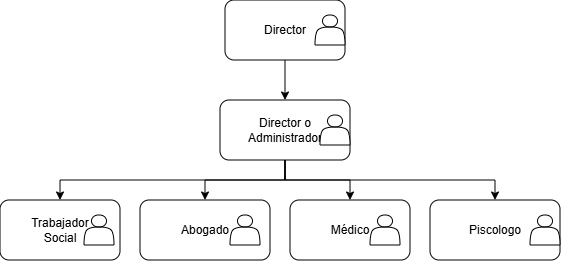
\includegraphics[width=.8\textwidth]{images/DiagraUsuarios}
		\caption{Organigrama de la Fundación Futuro con Derecho}
		\label{fig:organigrama}
	\end{center}
\end{figure}



%---------------------------------------------------------
\section{Procesos involucrados}

A continuación se describen los procesos operativos de la Fundación Futuro con Derecho 
que serán directamente afectados por la implementación del sistema SICORRE. Estos 
procesos fueron identificados a partir del análisis de la operación actual del equipo 
multidisciplinario.

\begin{figure}[htbp!]
	\begin{center}
		\includegraphics[width=.8\textwidth]{images/flujo}
		\caption{Mapa de procesos de la Fundación Futuro con Derecho.}
		\label{fig:mapaProcASIS}
	\end{center}
\end{figure}

\begin{description}
	\item[PR-01] \textbf{Control de acceso y autenticación.} Proceso mediante 
	el cual el personal de la fundación inicia y cierra sesión en el sistema 
	usando sus credenciales, validando su identidad mediante tokens JWT antes 
	de acceder a cualquier funcionalidad.
	
	\item[PR-02] \textbf{Gestión de usuarios y roles.} Proceso administrativo 
	mediante el cual la directora y la coordinadora registran nuevos integrantes 
	del equipo, asignan roles (administrador o especialista), modifican datos 
	de personal y gestionan el estatus de cada cuenta (activo, revocado 
	o eliminado).
	
	\item[PR-03] \textbf{Gestión de equipos multidisciplinarios.} Proceso de 
	configuración y administración de los equipos de trabajo, incluyendo el 
	alta de nuevos equipos, la asignación de integrantes con sus roles 
	correspondientes y el registro de fechas de ingreso y salida de cada 
	especialista.
	
	\item[PR-04] \textbf{Registro de datos del NNA.} Proceso mediante el cual 
	el trabajador social captura los datos personales, de ubicación y de 
	vulnerabilidad del niño, niña o adolescente conforme al Formato Único 
	de Datos (FUD) y la caja de herramientas, incluyendo CURP, domicilio 
	normalizado por SEPOMEX, estatus escolar, condición de migración, 
	idioma (INALI) y discapacidad.
	
	\item[PR-05] \textbf{Registro del hecho victimal.} Proceso mediante el 
	cual el trabajador social documenta los datos del hecho victimal asociado 
	al NNA, incluyendo el nombre de la víctima madre, fecha del hecho, datos 
	del expediente jurídico y descripción del delito, conforme a la FUD y 
	la caja de herramientas.
	
	\item[PR-06] \textbf{Registro y gestión del tutor del NNA.} Proceso de 
	captura y actualización de los datos del tutor legal o responsable del 
	NNA, incluyendo datos personales, domicilio normalizado por SEPOMEX, 
	idioma (INALI), enfermedades o padecimientos crónicos y datos de contacto.
	
	\item[PR-07] \textbf{Detección de duplicados.} Proceso automático mediante 
	el cual el sistema valida la CURP del NNA al momento del registro para 
	detectar expedientes duplicados y alertar al usuario antes de continuar 
	con la captura.
	
	\item[PR-08] \textbf{Apertura y gestión de expedientes.} Proceso de 
	creación, consulta, actualización y cierre de los expedientes asociados 
	a cada NNA, incluyendo el registro del folio FUD, el estatus del proceso, 
	la prioridad del caso y las fechas de apertura y seguimiento.
	
	\item[PR-09] \textbf{Registro de valoraciones multidisciplinarias.} 
	Proceso mediante el cual cada especialista del equipo (trabajador social, 
	abogado, psicólogo y médico) registra sus valoraciones, hallazgos, 
	dictámenes y medidas sugeridas sobre el expediente de un NNA, indicando 
	el área de evaluación y la fecha de la valoración.
	
	\item[PR-10] \textbf{Registro de derechos vulnerados.} Proceso de 
	identificación y documentación de los derechos específicos que han sido 
	vulnerados en cada caso, indicando el nombre del derecho, si se encuentra 
	activamente vulnerado y las observaciones pertinentes del equipo.
	
	\item[PR-11] \textbf{Vinculación de NNA con equipo multidisciplinario.} 
	Proceso mediante el cual el administrador o trabajador social asigna un 
	NNA registrado a un equipo multidisciplinario específico, habilitando el 
	acceso del equipo al expediente compartido del caso.
	
	\item[PR-12] \textbf{Consulta y búsqueda de información.} Proceso mediante 
	el cual cualquier integrante autorizado recupera la información de un NNA 
	o expediente específico, visualizando su estado actual, historial de 
	valoraciones y datos relevantes del caso de manera rápida y centralizada.
	
	\item[PR-13] \textbf{Control de fechas y calendario de expedientes.} 
	Proceso de registro y visualización de las fechas relevantes asociadas 
	a cada caso (apertura, consultas, diagnósticos, seguimientos), que permite 
	al equipo monitorear el avance temporal de los procesos de restitución 
	de derechos.
	
	\item[PR-14] \textbf{Gestión del catálogo de actores en materia de 
		derechos.} Proceso mediante el cual el administrador registra y mantiene 
	actualizado el catálogo de organizaciones gubernamentales, no 
	gubernamentales y personas físicas con capacidad de participar en la 
	restitución de derechos, incluyendo sus servicios, costos, ubicación, 
	horarios y datos de contacto.
	
	\item[PR-15] \textbf{Vinculación de actores con derechos vulnerados.} 
	Proceso mediante el cual el equipo multidisciplinario consulta el catálogo 
	de actores filtrando por municipio y tipo de servicio, para identificar 
	recursos disponibles que atiendan los derechos vulnerados de un NNA 
	específico.
	
	\item[PR-16] \textbf{Gestión de catálogos del sistema.} Proceso de 
	administración y consulta de los catálogos base del sistema, incluyendo 
	el catálogo de domicilios (SEPOMEX), el catálogo de idiomas y variantes 
	dialectales (INALI), el catálogo de tipos de discapacidad, el catálogo 
	de enfermedades y el catálogo de estados escolares, garantizando la 
	integridad y normalización de los datos capturados.
\end{description}





%---------------------------------------------------------
\section{Requerimientos de usuario}

Los requerimientos del usuario son los siguientes\FootnoteStatus:
\begin{requerimientosU}
	
	% ── CONTROL DE ACCESO ──────────────────────────────────────────
	\FRitem{RU-01}{Inicio de sesión al sistema}
	{El personal de la fundación debe poder autenticarse en el sistema 
		mediante correo electrónico y contraseña para acceder a las 
		funcionalidades correspondientes a su rol.}{1}{\DONE}
	
	\FRitem{RU-02}{Control de acceso por roles}
	{La directora, en colaboración con la coordinadora, debe poder 
		gestionar los accesos del personal al sistema, incluyendo el alta, 
		revocación y eliminación de cuentas de usuario, asignando un perfil 
		de rol a cada integrante del equipo multidisciplinario.}{1}{\DONE}
	
	\FRitem{RU-03}{Cierre de sesión}
	{El usuario debe poder cerrar su sesión en el sistema en cualquier 
		momento para proteger la confidencialidad de la información de los 
		NNA.}{2}{\DONE}
	
	% ── GESTIÓN DE PERSONAL ────────────────────────────────────────
	\FRitem{RU-04}{Registro de personal}
	{El administrador debe poder registrar nuevos integrantes del equipo 
		multidisciplinario en el sistema, capturando sus datos personales, 
		domicilio, rol y credenciales de acceso.}{1}{\DONE}
	
	\FRitem{RU-05}{Consulta de personal}
	{El administrador debe poder consultar el listado completo del 
		personal registrado en el sistema, visualizando su nombre, rol y 
		estatus de cuenta (activo o revocado).}{1}{\DONE}
	
	\FRitem{RU-06}{Modificación de datos de personal}
	{El administrador debe poder editar los datos personales y de acceso 
		de cualquier integrante del equipo registrado en el sistema.}{2}{\DONE}
	
	\FRitem{RU-07}{Revocación de acceso a usuario}
	{La directora o administrador debe poder revocar el acceso de un 
		integrante del equipo al sistema sin eliminar su historial de 
		actividad, conservando la trazabilidad de las valoraciones 
		registradas conforme a la normativa LGDNNA.}{1}{\DONE}
	
	\FRitem{RU-08}{Eliminación de usuario}
	{El administrador debe poder eliminar el registro de un usuario del 
		sistema cuando así se requiera, previa confirmación de la 
		acción.}{3}{\DONE}
	
	% ── MÓDULO DEL NNA ─────────────────────────────────────────────
	\FRitem{RU-09}{Registro de datos del NNA}
	{El trabajador social debe poder registrar los datos personales, de 
		ubicación y de vulnerabilidad de un niño, niña o adolescente con 
		base en el Formato Único de Datos (FUD) y la caja de herramientas, 
		incluyendo nombre completo, CURP, fecha de nacimiento, sexo, 
		nacionalidad, domicilio, estatus escolar, condición de migración, 
		lengua indígena y discapacidad.}{1}{\TODO}
	
	\FRitem{RU-10}{Registro del hecho victimal}
	{El trabajador social debe poder registrar los datos del hecho 
		victimal asociado al NNA, incluyendo el nombre de la víctima madre, 
		fecha del hecho, datos del expediente jurídico y descripción del 
		delito, conforme a lo establecido en la FUD y la caja de 
		herramientas.}{1}{\TODO}
	
	\FRitem{RU-11}{Registro de datos del tutor del NNA}
	{El trabajador social debe poder registrar los datos del tutor legal 
		o responsable del NNA, incluyendo sus datos personales, domicilio, 
		idioma, enfermedades o padecimientos relevantes y datos de 
		contacto.}{1}{\TODO}
	
	\FRitem{RU-12}{Detección de NNA duplicado}
	{El sistema debe alertar al usuario cuando se intente registrar un 
		NNA con una CURP ya existente en la base de datos, evitando la 
		duplicación de expedientes para la misma persona.}{1}{\TODO}
	
	\FRitem{RU-13}{Consulta de NNA}
	{Cualquier integrante autorizado del equipo debe poder buscar y 
		consultar la información de un NNA registrado en el sistema de 
		forma rápida, visualizando un resumen de su situación actual y el 
		historial de su expediente.}{1}{\TODO}
	
	\FRitem{RU-14}{Modificación de datos del NNA}
	{El trabajador social debe poder actualizar los datos personales y 
		de vulnerabilidad de un NNA previamente registrado cuando la 
		situación del caso así lo requiera.}{2}{\TODO}
	
	% ── MÓDULO DE EXPEDIENTES ──────────────────────────────────────
	\FRitem{RU-15}{Apertura de expediente}
	{El trabajador social debe poder crear un expediente de seguimiento 
		vinculado a un NNA registrado, asignando el folio FUD, el estatus 
		inicial del proceso, la prioridad del caso y la fecha de 
		apertura.}{1}{\TODO}
	
	\FRitem{RU-16}{Registro de valoraciones multidisciplinarias}
	{Cada especialista del equipo (trabajador social, abogado, psicólogo 
		y médico) debe poder registrar sus valoraciones, hallazgos, 
		dictámenes y medidas sugeridas sobre el expediente de un NNA, 
		indicando el área de evaluación y la fecha de la valoración.}{1}{\TODO}
	
	\FRitem{RU-17}{Registro de derechos vulnerados}
	{El equipo multidisciplinario debe poder registrar y actualizar los 
		derechos específicos que han sido vulnerados en cada caso, indicando 
		el nombre del derecho, si se encuentra activamente vulnerado y las 
		observaciones pertinentes.}{1}{\TODO}
	
	\FRitem{RU-18}{Consulta de expediente}
	{Cualquier integrante autorizado debe poder consultar el expediente 
		completo de un NNA, incluyendo todas las valoraciones registradas 
		por el equipo multidisciplinario y el historial de derechos 
		vulnerados.}{1}{\TODO}
	
	% ── MÓDULO DE ACTORES EN MATERIA DE DERECHOS ───────────────────
	\FRitem{RU-19}{Registro de actores en materia de derechos}
	{El administrador debe poder registrar en el sistema organizaciones 
		gubernamentales, no gubernamentales y personas físicas que cuenten 
		con capacidades para participar en la restitución de derechos de los 
		NNA, incluyendo sus datos de contacto, ubicación, horarios, 
		servicios ofrecidos, costos y requisitos.}{1}{\TODO}
	
	\FRitem{RU-20}{Consulta de actores por municipio y tipo de servicio}
	{El equipo multidisciplinario debe poder consultar el catálogo de 
		actores en materia de derechos filtrando por municipio y tipo de 
		servicio, con el fin de identificar recursos disponibles para 
		atender los derechos vulnerados de un NNA específico.}{1}{\TODO}
	
	% ── CATÁLOGOS ──────────────────────────────────────────────────
	\FRitem{RU-21}{Registro de domicilios mediante catálogo SEPOMEX}
	{Todos los domicilios capturados en el sistema (NNA, tutor, usuarios 
		y actores) deben registrarse mediante el catálogo oficial de códigos 
		postales de SEPOMEX, garantizando la correcta asociación de colonia, 
		municipio y entidad federativa.}{2}{\TODO}
	
	\FRitem{RU-22}{Registro de idiomas conforme al catálogo INALI}
	{El sistema debe permitir registrar el conocimiento de idiomas del 
		NNA y su tutor conforme al catálogo oficial del Instituto Nacional 
		de Lenguas Indígenas (INALI), especificando idioma, variante 
		dialectal y nivel de dominio.}{2}{\TODO}
	
	\FRitem{RU-23}{Registro de discapacidades}
	{El sistema debe permitir registrar las discapacidades del NNA y su 
		tutor especificando el tipo de discapacidad y el grado de 
		dependencia, conforme a los estándares de clasificación 
		aplicables.}{2}{\TODO}
	
	\FRitem{RU-24}{Registro de enfermedades y padecimientos}
	{El sistema debe permitir registrar los padecimientos y enfermedades 
		del NNA y su tutor, indicando si son crónicas, si están controladas 
		y el tratamiento en curso, conforme a los catálogos de enfermedades 
		aplicables.}{2}{\TODO}
	
	% ── EQUIPOS MULTIDISCIPLINARIOS ────────────────────────────────
	\FRitem{RU-25}{Gestión de equipos multidisciplinarios}
	{El administrador debe poder crear y gestionar equipos 
		multidisciplinarios, asignando integrantes con sus respectivos roles 
		y registrando fechas de ingreso y salida de cada especialista 
		dentro del equipo.}{2}{\TODO}
	
	\FRitem{RU-26}{Asignación de NNA a equipo multidisciplinario}
	{El administrador o trabajador social debe poder asignar un NNA 
		registrado a un equipo multidisciplinario específico para que los 
		integrantes de dicho equipo puedan visualizar y actualizar su 
		expediente.}{1}{\TODO}
	
	% ── CALENDARIO ─────────────────────────────────────────────────
	\FRitem{RU-27}{Consulta de calendario de expedientes}
	{El equipo multidisciplinario debe poder visualizar un calendario 
		con las fechas de apertura, consultas, diagnósticos y seguimientos 
		de los casos activos, facilitando el control temporal de los 
		procesos de restitución de derechos.}{2}{\TODO}
	
\end{requerimientosU}
%---------------------------------------------------------

\section{Especificación de plataforma}

El sistema SICORRE es una aplicación de tipo web con arquitectura Cliente-Servidor, 
diseñada para operar en red local dentro de las instalaciones de la Fundación Futuro 
con Derecho, con capacidad de despliegue en la nube para pruebas y acceso remoto 
autorizado. A continuación se describe la plataforma tecnológica requerida.

\begin{description}
	
	\item[Tipo de sistema:] Aplicación web de arquitectura Cliente-Servidor. 
	El Front End es una aplicación React/NextJS que se ejecuta en el navegador 
	del usuario. El Back End es una API REST desarrollada con FastAPI (Python) 
	que procesa las solicitudes y gestiona la lógica del negocio. La base de 
	datos es relacional (PostgreSQL) y almacena toda la información del sistema. 
	La comunicación entre capas se realiza mediante peticiones HTTP/HTTPS con 
	intercambio de datos en formato JSON y autenticación por tokens JWT.
	
	\item[Software requerido en el servidor:] 
	\begin{itemize}
		\item Sistema operativo: Ubuntu 24.04 LTS (Linux).
		\item Python 3.12 o superior con entorno virtual \texttt{venv}.
		\item Framework Back End: FastAPI con servidor ASGI Uvicorn.
		\item Gestor de dependencias: \texttt{pip} con archivo 
		\texttt{requirements.txt}.
		\item Motor de base de datos: PostgreSQL 16.
		\item Administrador de base de datos: pgAdmin 4 (opcional, para 
		administración local).
		\item Node.js v24 LTS (instalado mediante NVM) para compilación 
		del Front End.
		\item Framework Front End: Next.js 16 con React.
		\item Gestor de paquetes: npm.
		\item Control de versiones: Git.
	\end{itemize}
	
	\item[Software requerido en el cliente:] 
	\begin{itemize}
		\item Navegador web moderno: Google Chrome 120+, Mozilla Firefox 
		120+, Microsoft Edge 120+ o equivalente con soporte para ES2020 
		y CSS Grid.
		\item No se requiere instalación de software adicional en los 
		equipos cliente, ya que la interfaz se sirve íntegramente desde 
		el navegador.
	\end{itemize}
	
	\item[Hardware requerido en el servidor:]
	\begin{itemize}
		\item Procesador: CPU de 64 bits, mínimo 2 núcleos a 2.0 GHz 
		(recomendado 4 núcleos a 2.5 GHz o superior).
		\item Memoria RAM: mínimo 4 GB (recomendado 8 GB).
		\item Almacenamiento: mínimo 20 GB de espacio en disco duro 
		(recomendado SSD de 50 GB para mejor rendimiento de PostgreSQL).
		\item Interfaz de red: tarjeta de red Ethernet 100/1000 Mbps.
	\end{itemize}
	
	\item[Hardware requerido en los equipos cliente:]
	\begin{itemize}
		\item Procesador: cualquier CPU de 64 bits con velocidad mínima 
		de 1.5 GHz.
		\item Memoria RAM: mínimo 2 GB.
		\item Resolución de pantalla: mínimo 1280 $\times$ 720 píxeles.
		\item Dispositivo de entrada: teclado y ratón o pantalla táctil.
	\end{itemize}
	
	\item[Servicios requeridos:]
	\begin{itemize}
		\item \textbf{Conectividad:} Red local (LAN) o conexión a Internet 
		para acceso al sistema desplegado en Railway (Back End) y Vercel 
		(Front End). Ancho de banda mínimo recomendado: 10 Mbps.
		
		\item \textbf{Seguridad:} Autenticación mediante tokens JWT con 
		expiración configurable. Cifrado de contraseñas con hash seguro 
		(bcrypt). Comunicación cifrada mediante HTTPS/TLS en el entorno 
		de producción.
		
		\item \textbf{Despliegue en la nube:}
		\begin{itemize}
			\item \textbf{Railway:} Plataforma de despliegue para el 
			servidor FastAPI y la instancia de PostgreSQL, con gestión 
			de variables de entorno y logs en tiempo real.
			\item \textbf{Vercel:} Plataforma de despliegue para el 
			Front End NextJS, con red de distribución de contenido (CDN) 
			global y previsualización por ramas de desarrollo.
		\end{itemize}
		
		\item \textbf{Respaldo de datos:} Se recomienda configurar 
		respaldos automáticos periódicos de la base de datos PostgreSQL 
		mediante los mecanismos de backup provistos por Railway, o 
		mediante \texttt{pg\_dump} en instalaciones locales, con 
		frecuencia mínima diaria.
		
		\item \textbf{Control de versiones y despliegue continuo:} 
		Repositorio Git con integración a Railway y Vercel para despliegue 
		automático (Continuous Deployment) ante cambios en la rama 
		principal del proyecto.
	\end{itemize}
	
\end{description}

\begin{figure}[htbp!]
	\begin{center}
		\fbox{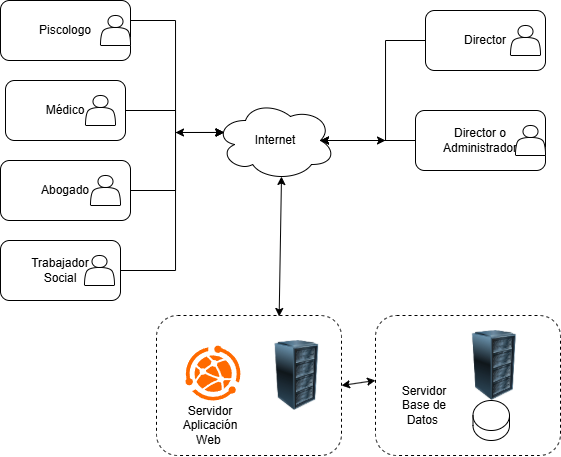
\includegraphics[width=.6\textwidth]{images/arquitectura}}
		\caption{Arquitectura del sistema.}
		\label{fig:arquitectura}
	\end{center}
\end{figure}


